\section{Application Layer}

\subsection{DNS}

Rekursive Abfrage: Server führt alle notwendigen Subqueries zur vollständigen
Auflösung aus.

Nicht-Rekursive Abfrage: Server liefert nur den nächsten zuständigen Name
Server. Nach dem Prinzip "Frag einmal dort nach".

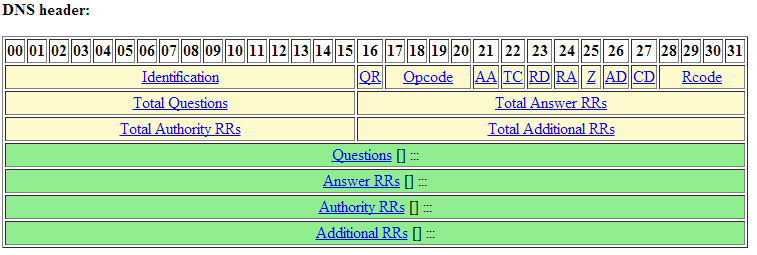
\includegraphics[width=\textwidth]{media/DNSHeader.png}

\subsection{FTP}

\subsubsection{Connection Modi}

\textbf{Aktiv:} Der Server baut die Datenkanal-Verbindung zum Client auf

\textbf{Passiv:} Der Client baut die Verbindung für den Datenkanal zum Server auf. Der
Server ist nur "listening".

\subsubsection{Beispielverbindung}

\begin{verbatim}
USER jonas
PASS jonas
PASV
227: Entering Passive Mode (xxx,xxx,xxx,xxx,y,z)
// Port = 256*y+z
LIST
\end{verbatim}

\subsubsection{File Transfer Mode}

Im ASCII Mode werden die CR/LF für die jeweilige Zielplattform konvertiert. Im
Binary Mode wird nichts konvertiert.

\subsection{HTTP}

\subsubsection{Persistent HTTP}

keep-alive Header, TCP Verbindung bleibt für mehrere Requests erhalten.

\subsubsection{Conditional Get}

\textbf{Header für Cache Control}

\begin{itemize}
	\item if-match
	\item if-none-match
	\item if-modified-since
	\item if-range
\end{itemize}

\textbf{ETag}

Bei der ersten Anfrage einer Ressource sendet der Server einen für diese
Ressource spezifischen ETag-Wert im ETag-Header-Feld, der vom Client zusammen
mit der Ressource lokal gespeichert wird. (Abb.1) Bei einer erneuten Anfrage
derselben Ressource sendet der Client in dem Header-Feld If-None-Match den zuvor
gespeicherten ETag-Wert mit. (Abb.2) Auf der Server-Seite wird nun der gesendete
ETag-Wert mit dem aktuellen verglichen und bei Übereinstimmung mit dem
Statuscode 304 beantwortet. (Abb.3) Die Daten der Ressource werden in diesem
Fall nicht mitgeschickt und der Client verwendet die lokal gespeicherten
Daten.

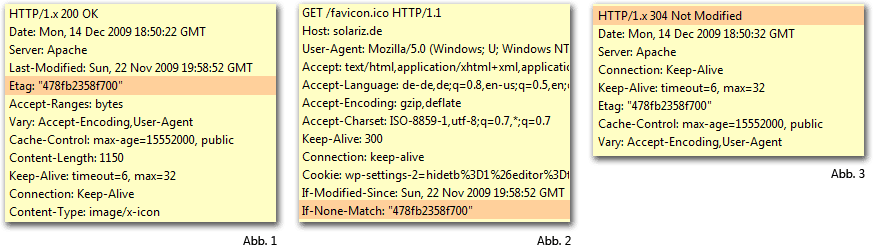
\includegraphics[width=\textwidth]{media/etag_beispiele.png}
